\section{Synchronizing Shapes with \prism}
\label{sec:prism}

\subsection{Projection of language}
\td{Languages aren't actually projected (they could, but not our focus).}
\td{I do not get the sectioning. Actually I would rename Section 2 to something else (conceptual something\dots), and rename 2.1 as Section 3 with current Section 2 title without subsections}

Whenever an incarnation of a model is updated, its containing LV transforms the changes to a patch and ships its to \prism.
\prism then propagates the patch to every other incarnation of the same model using a simple matrix that keeps track of which model every incarnation is a projection of.
Every LV is then responsible for updating its own incarnation by interpreting the patch.

\begin{figure}[bt]
	\centering
	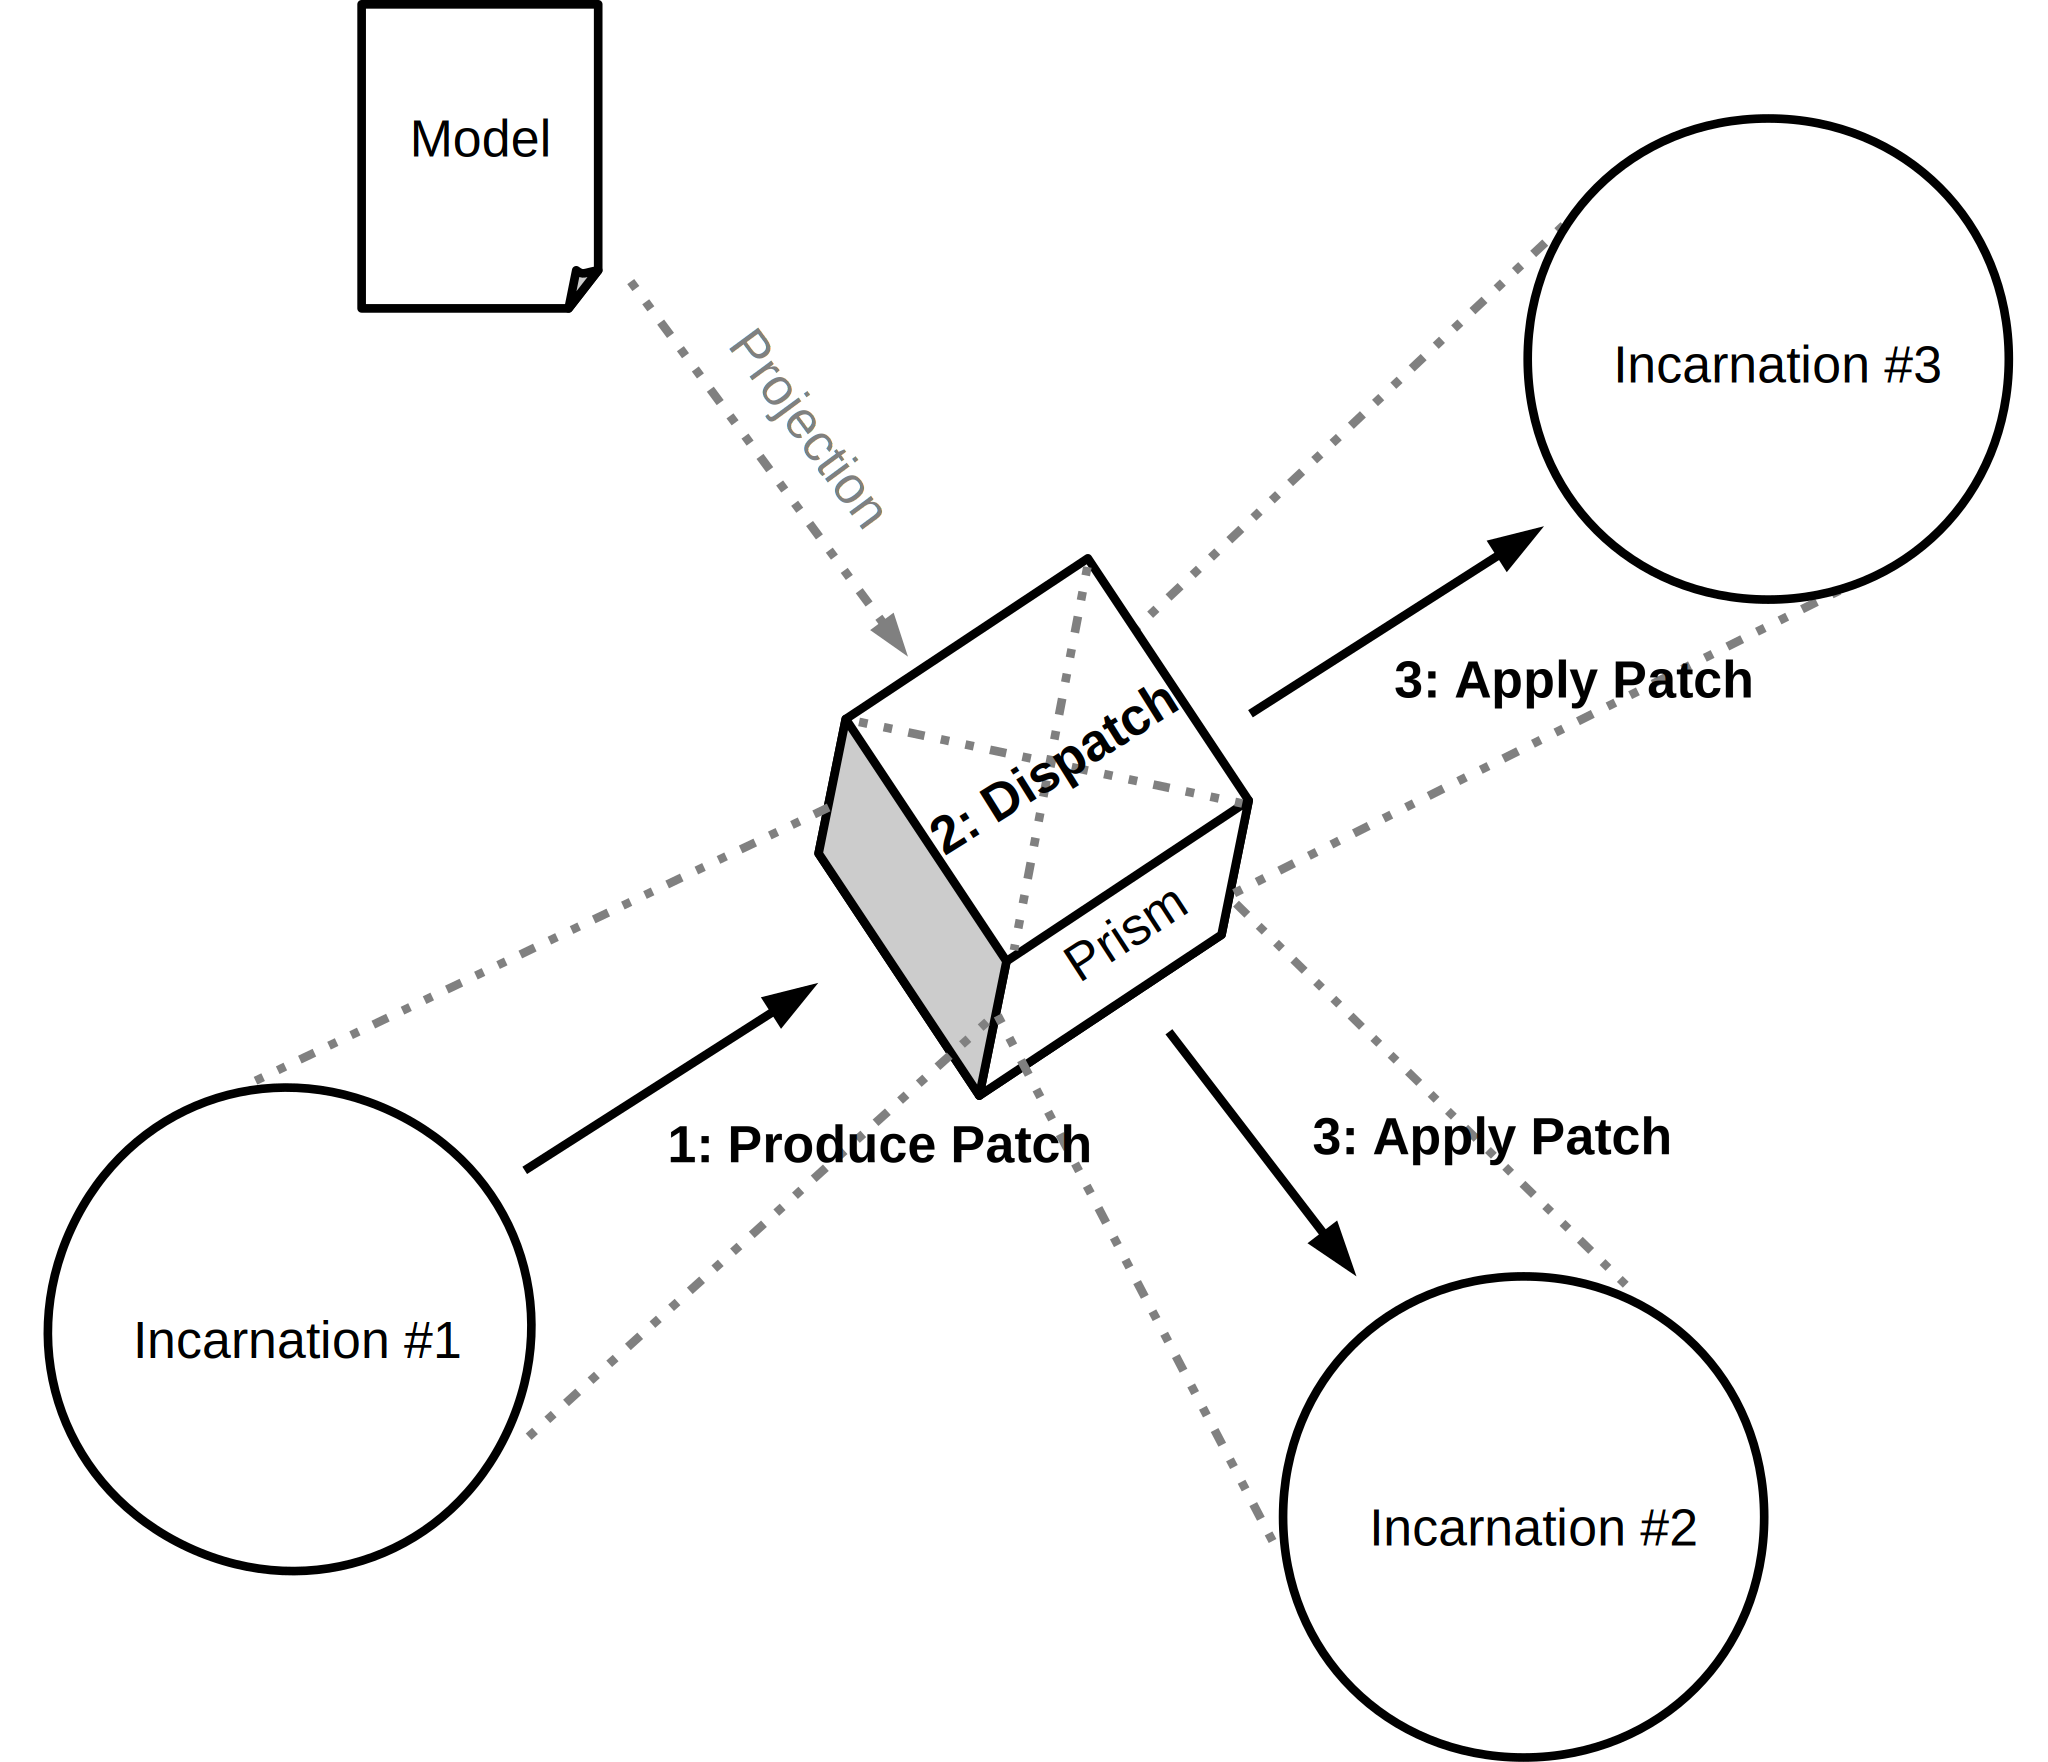
\includegraphics[width=.6\columnwidth]{figures/prism}
	\caption{Using \prism to synchronize Incarnation \#1 with two other incarnations of the same model}
	\label{fig:prism}
\end{figure}

The key underlying idea of our approach is to provide the capability, at any time, to ``project'' a given model in any of its shapes and to synchronize those shapes whenever one of them is updated.
We enable the projection of a given model as an ADT value, to be manipulated in the Rascal TS, or as an Ecore model, to be manipulated in the EMF TS.
\fc{LV instead of TS (in the whole paper?)}

Our approach keeps the TS fully independent and builds a communication bus between them.
Both representations of the same model in various TS are kept in memory to allow online synchronization of the same models manipulated by different stakeholders in different shapes.
When a changes occurs on either side, this side is responsible for generating a \emph{patch} (aka. \de or edit script~\cite{rozen2017towards}), that stores the changes on the model that have been realized on this side.
The communication bus then ships this patch to all the other sides.
Every side interprets the patch in its own way to keep the representation synchronized.
On the EMF side, for instance, the patch is interpreted as a set of changes that impact an Ecore model, while on the Rascal side it is interpreted as a set of changes that impact a value conforming to the ADT defining the AS of the language.
\fc{sides = LVs ?}

It is important to note that each TS may want to preserve certain information across the patches that are specific to the TS.
A textual editor in Rascal, for instance, needs to keep some of the parsing information to maintain layout whenever patches are applied.
So it should be possible to apply the patch while maintaining the extra information specific to a given TS.

Automatically generating language implementations in different TS is beyond the scope of this paper.\footnote{Indeed, this would actually require to build some kind of BX between all AS formalisms; so, nope!} Instead, given various shapes of a language, implemented by hand, we provide the means to automatically synchronize the projections of a model.

\begin{lstlisting}[label=lst:delta-adt, caption={CRUD-like \ds structure definition in Rascal}, language=Rascal]
@doc{A patch consists of a sequence of edits}
alias Patch = tuple[Id root, Edits edits];

@doc{Edits are operations attached to object identities}
alias Edits = lrel[Id obj, Edit edit];

data Edit
= put(str field, value val)
| unset(str field)
| ins(str field, int pos, value val)
| del(str field, int pos)
| create(str class) 
| destroy();
\end{lstlisting}

It is important to note that ``projections'' have no relation whatsoever with projectional editing.
A projection denotes the incarnation of a model in a particular shape of a language.
In \Cref{fig:motivating-fsm}, the lower part depicts three projections of the same \texttt{Button} state machine model in three shapes of the FSM language.
We use the term ``language'' to refer to the specification of a language independently from its realization in a given TS.
A concrete implementation of a language is a ``shape''.
An instance of a shape, \ie~a particular model in a particular TS, is a ``projection'' of a ``virtual'' model.
Metamorphic synchronization refers to the ability to synchronize the projections of a given model for every shapes of a language.
